%%%%%%%%%%%%%%%%%%%%%%%%%%%%%%% beamer %%%%%%%%%%%%%%%%%%%%%%%%%%%%%%%%%%%%%%%%%%%%%%%%%
% To run - pdflatex filename.tex
%      acroread filename.pdf
%%%%%%%%%%%%%%%%%%%%%%%%%%%%%%%%%%%%%%%%%%%%%%%%%%%%%%%%%%%%%%%%%%%%%%%%%%%%%%%%%%%%%%%%

\documentclass[compress,oilve]{beamer}
\mode<presentation>

\usetheme[]{CambridgeUS}
% other themes: AnnArbor, Antibes, Bergen, Berkeley, Berlin, Boadilla, boxes, CambridgeUS, Copenhagen, Darmstadt, default, Dresden, Frankfurt, Goettingen,
% Hannover, Ilmenau, JuanLesPins, Luebeck, Madrid, Maloe, Marburg, Montpellier, PaloAlto, Pittsburg, Rochester, Singapore, Szeged, classic

\usecolortheme{beaver}
% color themes: albatross, beaver, beetle, crane, default, dolphin,  fly, lily, orchid, rose, seagull, seahorse, sidebartab, whale, wolverine

\usefonttheme{professionalfonts}
% font themes: default, professionalfonts, serif, structurebold, structureitalicserif, structuresmallcapsserif


\hypersetup{pdfpagemode=FullScreen} % makes your presentation go automatically to full screen

% define your own colors:
\definecolor{Red}{rgb}{1,0,0}
\definecolor{Blue}{rgb}{0,0,1}
\definecolor{Green}{rgb}{0,1,0}
\definecolor{magenta}{rgb}{1,0,.6}
\definecolor{lightblue}{rgb}{0,.5,1}
\definecolor{lightpurple}{rgb}{0.8, 0.6, 0.9}
\definecolor{gold}{rgb}{.6,.5,0}
\definecolor{orange}{rgb}{1,0.4,0}
\definecolor{hotpink}{rgb}{1,0,0.5}
\definecolor{newcolor2}{rgb}{.5,.3,.5}
\definecolor{newcolor}{rgb}{0,.3,1}
\definecolor{newcolor3}{rgb}{1,0,.35}
\definecolor{darkgreen1}{rgb}{0, .35, 0}
\definecolor{darkgreen}{rgb}{0, .6, 0}
\definecolor{darkred}{rgb}{.75,0,0}
\definecolor{skyblue}{HTML}{75bbfd}

\definecolor{olive}{cmyk}{0.64,0,0.95,0.4}
\definecolor{purpleish}{cmyk}{0.75,0.75,0,0}

% can also choose different themes for the "inside" and "outside"

% \usepackage{beamerinnertheme_______}
% inner themes include circles, default, inmargin, rectangles, rounded

% \usepackage{beamerouterthemesmoothbars}
% outer themes include default, infolines, miniframes, shadow, sidebar, smoothbars, smoothtree, split, tree


\useoutertheme[subsection=true, height=40pt]{smoothbars}

% to have the same footer on all slides
%\setbeamertemplate{footline}[text line]{STUFF HERE!}
\setbeamertemplate{footline}[text line]{} % makes the footer EMPTY
% include packages
%

%show the page numbers in footnote
%\addtobeamertemplate{navigation symbols}{}{%
%	\usebeamerfont{footline}%
%	\usebeamercolor[fg]{footline}%
%	\hspace{1em}%
%	\insertframenumber/\inserttotalframenumber
%}

\setbeamercolor{footline}{fg=purpleish}
\setbeamerfont{footline}{series=\bfseries}

%add color to curent subsection
\setbeamertemplate{section in head/foot}{\hfill\tikz\node[rectangle, fill=darkred, rounded corners=1pt,inner sep=1pt,] {\textcolor{white}{\insertsectionhead}};}
\setbeamertemplate{section in head/foot shaded}{\textcolor{darkred}{\hfill\insertsectionhead}}

% Remove bullet of subsections
\setbeamertemplate{headline}
{%
	\begin{beamercolorbox}{section in head/foot}
		\insertsectionnavigationhorizontal{\textwidth}{}{}
	\end{beamercolorbox}%
}


% modify headlline, specially headline size
\setbeamertemplate{headline}{%
	\leavevmode%
	\hbox{%
		\begin{beamercolorbox}[wd=\paperwidth,ht=3.5ex,dp=1.125ex]{palette quaternary}%
			\insertsectionnavigationhorizontal{\paperwidth}{}{\hskip0pt plus1filll}
		\end{beamercolorbox}%
	}
}

\setbeamertemplate{footline}{%
	\leavevmode%
	\hbox{\begin{beamercolorbox}[wd=.5\paperwidth,ht=2.5ex,dp=1.125ex,leftskip=.3cm plus1fill,rightskip=.3cm]{author in head/foot}%
			\usebeamerfont{author in head/foot}\insertshortauthor ~ \insertshortinstitute
		\end{beamercolorbox}%
		\begin{beamercolorbox}[wd=.5\paperwidth,ht=2.5ex,dp=1.125ex,leftskip=.3cm,rightskip=.3cm plus1fil]{title in head/foot}%
			\usebeamerfont{title in head/foot}\insertshorttitle\hfill\insertframenumber\,/\,\inserttotalframenumber
	\end{beamercolorbox}}%
	\vskip0pt%
}


%\setbeamertemplate{navigation symbols}{}

\title{Support Vector Machines}
\author{ML Instruction Team, Fall 2022}
\institute[]{CE Department \newline  Sharif University of Technology \newline \newline \newline
	Ali Sharifi-Zarchi \newline
	Behrooz Azarkhalili \newline
	Alireza Gargoori Motlagh}
\date[\today]{}
%\titlegraphic{\includegraphics[scale=.35]{example-image}}



%Write \usepackage{etex} just after the \documentclass line (it should be the first loaded package).
\usepackage{etex}
\usepackage{subcaption}
\usepackage{multicol}
\usepackage{amsmath}
\usepackage{epsfig}
\usepackage{graphicx}
\usepackage{amsmath}
\usepackage[all,knot]{xy}
\xyoption{arc}
\usepackage{url}
\usepackage{multimedia}
\usepackage{hyperref}
\hypersetup{colorlinks,linkcolor=blue,citecolor=redorange,urlcolor=darkred}
\usepackage{multirow}
\usepackage[font={scriptsize}]{caption}
\usepackage{pgf}
\usepackage{fontspec}
%\setsansfont[Scale=MatchLowercase, BoldFont = * Bold, ItalicFont = * Italic]{Caladea}

%\usepackage{enumitem,xcolor}
%\newcommand{\labelitemi}{$\blacksquare$}
%\newcommand{\labelitemii}{$\diamond$}
%\newcommand{\labelitemiii}{$\square$}
%\newcommand{\labelitemiv}{$\ast$}
%\setbeamercolor*{item}{fg=red}


\usefonttheme{professionalfonts} 
\setbeamertemplate{itemize item}{\color{skyblue}$\blacksquare$}
\setbeamertemplate{itemize subitem}{\color{hotpink}$\blacktriangleright$}
\setbeamertemplate{itemize subsubitem}{\color{orange}$\bullet$}


\usepackage{anyfontsize}
\usepackage{t1enc}
\usepackage{tikz}
\usetikzlibrary{calc,trees,positioning,arrows,chains,shapes.geometric,decorations.pathreplacing,decorations.pathmorphing,shapes,matrix,shapes.symbols}



\newtheorem{proposition}[theorem]{Proposition}
\newtheorem{remark}[theorem]{Remark}
\newtheorem{assumption}[theorem]{Assumption}

\usepackage{fontspec,unicode-math}
\setmainfont[Scale=0.9]{Consolas}
%\setmonofont[Scale=0.9]{Monaco}
\setsansfont[Scale=1]{Times New Roman}


%\usepackage{smartdiagram}
%\usesmartdiagramlibrary{additions}
%%%%%%%%%%%%%%%%%%%%%%%%%%%%%%%%%%%%%%%%%%%%%%%%%%%%%%%%%%%%%%%%%%%%%%%%%%%%%%%%%%%%%%%%%%%%
%%%%%%%%%%%%%%%%%%%%%%%%%%%%%% Title Page Info %%%%%%%%%%%%%%%%%%%%%%%%%%%%%%%%%%%%%%%%%%%
%%%%%%%%%%%%%%%%%%%%%%%%%%%%%%%%%%%%%%%%%%%%%%%%%%%%%%%%%%%%%%%%%%%%%%%%%%%%%%%%%%%%%%%%%%


%%%%%%%%%%%%%%%%%%%%%%%%%%%%%%%%%%%%%%%%%%%%%%%%%%%%%%%%%%%%%%%%%%%%%%%%%%%%%%%%%%%%%%%%%%
%%%%%%%%%%%%%%%%%%%%%%%%%%%%%% Begin Your Document %%%%%%%%%%%%%%%%%%%%%%%%%%%%%%%%%%%%%%%
%%%%%%%%%%%%%%%%%%%%%%%%%%%%%%%%%%%%%%%%%%%%%%%%%%%%%%%%%%%%%%%%%%%%%%%%%%%%%%%%%%%%%%%%%%
\begin{document}
	
	%%%%%%%%%%%%%%%%%%%%%%%%%%%%%%%%%%%%%%%%%%%%%%%%%%%%%%%%%%%%%%%%%%%%%%%%%%%%%%%%%%%%%%%%%%
	\fontsize{9}{9}
	\begin{frame}[noframenumbering, plain]
		\titlepage
	\end{frame}
	
	%%%%%%%%%%%%%%%%%%%%%%%%%%%%%%%%%%%%%%%%%%%%%%%%%%%%%%%%%%%%%%%%%%%%%%%%%%%%%%%%%%%%%%%%%%
	\section{Introduction}
	%%%%%%%%%%%%%%%%%%%%%%%%%%%%%%%%%%%%%%%%%%%%%%%%%%%%%%%%%%%%%%%%%%%%%%%%######
	\frame{\frametitle{Intuition: Margins}
		
		
		\begin{itemize}
			\item Separating Hyperplane
			\begin{figure}
				\centering
				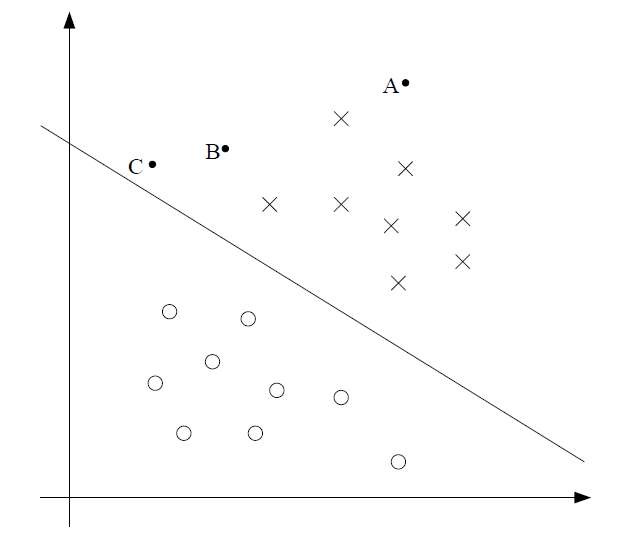
\includegraphics[scale=0.4]{images/separating_hyperplane.png}
			\end{figure}
			
			\item 
			Our confidence about the prediction of classes of A, B and C relies on their distance from decision boundary. \newline
			
			\item 
			We try to find the optimal hyperplane that separates the classes in the feature space.
		\end{itemize}	
		
	}
	
	%%%%%%%%%%%%%%%%%%%%%%%%%%%%%%%%%%%%%%%%%%%%%%%%%%%%%%%%%%%%%%%%%%%%%%%%%%%%%%%%%%%%%%%%%%%%
	\frame{\frametitle{Hyperplane}
		
		
		\begin{itemize}
			\item \textbf {Hyperplane}: A hyperplane in \textit p dimensions is a flat affine subspace of dimension \textit {p-1}: \newline
			
			$$\beta_0 + \beta_1 X_1 + \beta_2 X_2 + ... + \beta_p X_p = 0$$ \newline
			
			\item The vector $\beta = (\beta_1, \beta_2, ..., \beta_p)$ is called the normal vector -- it points in a direction orthogonal to the surface of the defined hyperplane. \newline 
			
			
			\item If $f(X) = \beta_0 + \beta_1 X_1 + \beta_2 X_2 + ... + \beta_p X_p = \beta^T X + \beta_0$, then $f(X)$ divides the \textit p-dimensional feature space into two half-spaces ($f(X) > 0$ for one side and $f(X) < 0$ for the other side). \newline \newline
			
			\item So if we code $Y^{(i)} \in \{\pm 1\}$, then $\forall i$
			 $$Y^{(i)}f(X^{(i)}) > 0$$
		\end{itemize}	
		
	}
	%%%%%%%%%%%%%%%%%%%%%%%%%%%%%%%%%%%%%%%%%%%%%%%%%%%%%%%%%%%%%%%%%%%
	\section{Maximal Margin Classifier}
	%%%%%%%%%%%%%%%%%%%%%%%%%%%%%%%%%%%%%%%%%%%%%%%%%%%%%%%%%%%%%%%%%%%
	\frame{\frametitle{Maximal Margin Classifier}
		
		\begin{itemize}
	
			\begin{figure}
				\centering
				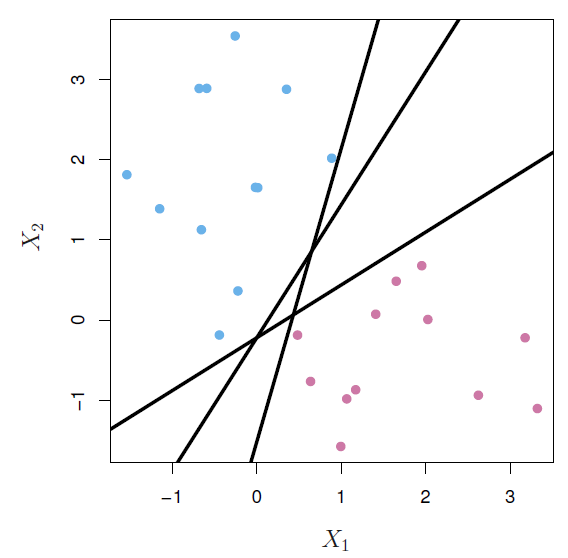
\includegraphics[scale=0.35]{images/possible_hyperplanes.png}
			\end{figure}
		
			\item \textbf{Maximal(Optimal) Separating  Hyperplane}: The separating hyperplane with the biggest margin between the classes.
			
			\begin{equation}
				\begin{aligned}
					\max_{\beta_0, \beta_1,...,\beta_p,‌M} & M\\
					\textrm{s.t.} \quad & \sum_{j=1}^{p} \beta_j ^2 = 1\\
					 & y^{(i)}(\beta^T x^{(i)} + \beta_0) > M \quad \forall i\in \{1,2,...,N\}\\
				\end{aligned}
			\end{equation}
			
		\end{itemize}	
		
	}
	
	\frame{\frametitle{Maximal Margin Classifier: Quadratic Program}
		
		
		\begin{itemize}
			\item Eq.(1) can be rephrased as a convex quadratic problem and be solved efficiently using QP solvers.
			\newline
			\item
			(Euclidean) distance between two hyperplanes \newline
			
			$$\mathcal{H}_1 = \{x | \beta^T x + \beta_0 = 1\} \quad \quad
			\mathcal{H}_2 = \{x | \beta^T x + \beta_0 = -1\}$$ \vspace{2mm}
			
			is \textbf {dist($\mathcal{H}_1, \mathcal{H}_2$)} = 2/$||\beta||_2$ \newline
			
			\begin{equation}
				\begin{aligned}
					\min_{\beta,\beta_0} \quad & \frac{1}{2}||\beta||_2 ^2\\
					\textrm{s.t.} \quad & y^{(i)}(\beta^T x^{(i)} + \beta_0) \geq 1 \quad \forall i \in {1,2,...,N}\\
				\end{aligned}
			\end{equation}
			\qquad
			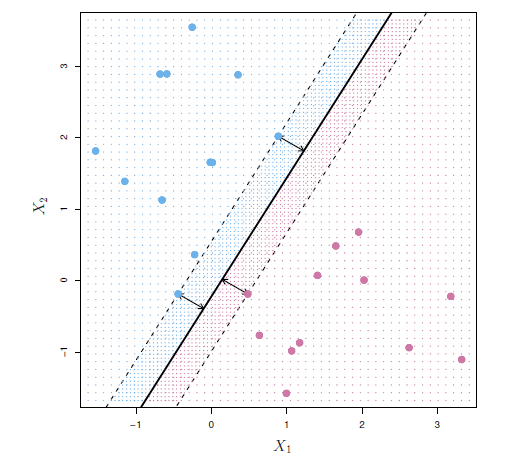
\includegraphics[scale=0.4]{images/maximal_hyperplane.png}
			
			
			%\begin{figure}
				%\centering
				%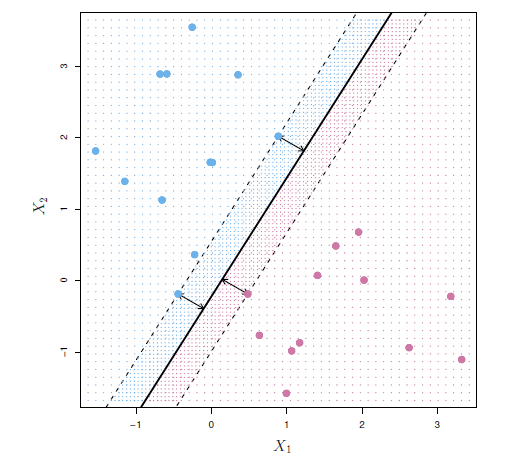
\includegraphics[scale=0.35]{images/maximal_hyperplane.png}
			%\end{figure}
		\end{itemize}	
		
	}

	%%%%%%%%%%%%%%%%%%%%%%%%%%%%%%%%%%%%%%%%%%%%%%%%%%%%%%%%%%%%%%%%%%%
	\section{Support Vector Classifier}
	%%%%%%%%%%%%%%%%%%%%%%%%%%%%%%%%%%%%%%%%%%%%%%%%%%%%%%%%%%%%%%%%%%%
	\frame{\frametitle{Non-linear Separable Data}
		
		\begin{itemize}
			
			\item In most cases however, the data are not linearly separable unless $N < p$ .
			\newline
			\begin{figure}
				\centering
				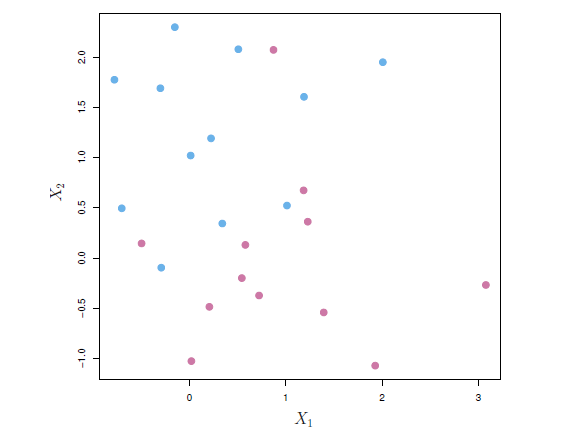
\includegraphics[scale=0.5]{images/non_separable.png}
			\end{figure}
			
		\end{itemize}	
		
	}

	\frame{\frametitle{Noisy Data}
		
		\begin{itemize}
			
			\item Sometimes the data are linearly separable, but noisy. This can lead to a poor solution for the maximal margin classifier. Also, hard-margin classifier is sensitive to outliers.
			\begin{figure}
				\centering
				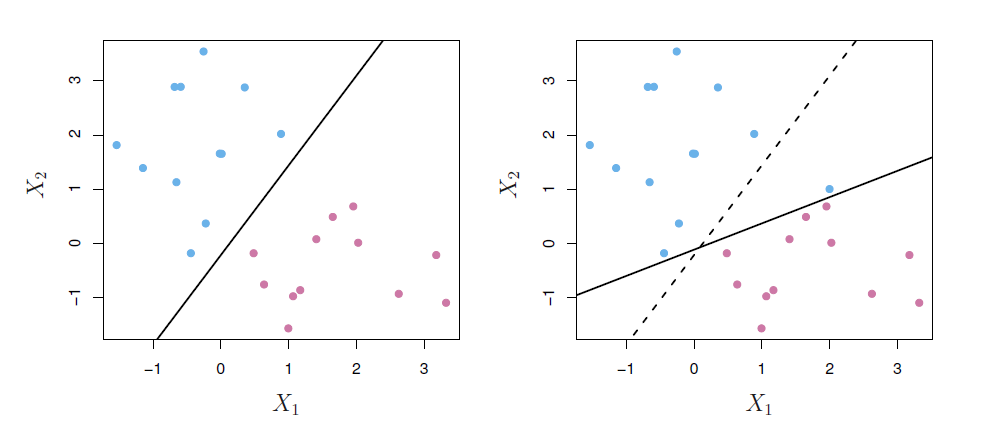
\includegraphics[scale=0.5]{images/noisy_data.png}
			\end{figure}
		
			\item The \textcolor{Blue}{\textit {support vector classifier}} maximizes a \textcolor{Blue}{\textit {soft}} margin.
			
		\end{itemize}	
		
	}


	\frame{\frametitle{Support Vector Classifier(Soft Margin Classifier)}
		
		\begin{itemize}
			
			\item Allowing some samples to violate the margin, with \textit {slack variables}, in a controlled manner.
			\begin{figure}
				\centering
				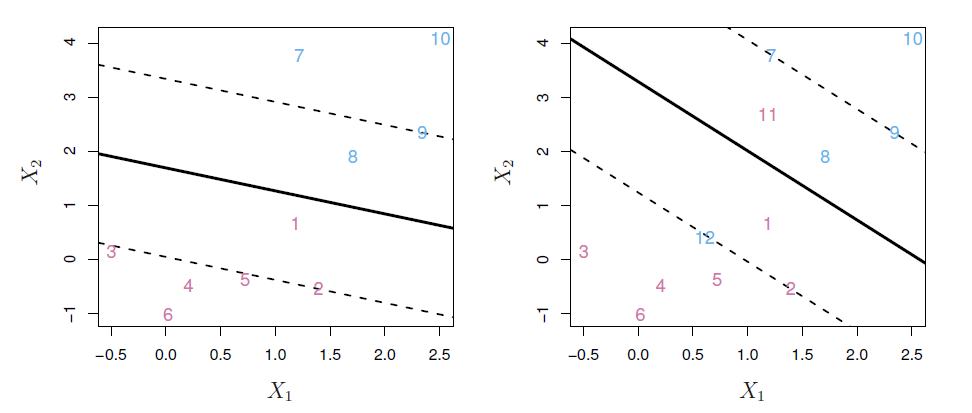
\includegraphics[scale=0.5]{images/support_vector_classifier.png}
			\end{figure}
			
			\begin{equation}
				\begin{aligned}
					\min_{\beta,\beta_0,\xi} \quad & \frac{1}{2}||\beta||_2 ^2+C\sum_{i=1}^{N}{\xi_{i}}\\
					\textrm{s.t.} \quad & y^{(i)}(\beta^T x^{(i)} + \beta_0) \geq 1-\xi_{i}\\
					&\xi_i\geq0 \quad \forall i \in \{1,2,...,N\}   \\
				\end{aligned}
			\end{equation}
			
		\end{itemize}	
		
	}


	\frame{\frametitle{Effect of Regularization Parameter}
		
		\begin{itemize}
			
			\item \textit C is a regularization parameter that controls the bias-variance trade-off of the support vector classifier.
			\begin{figure}
				\centering
				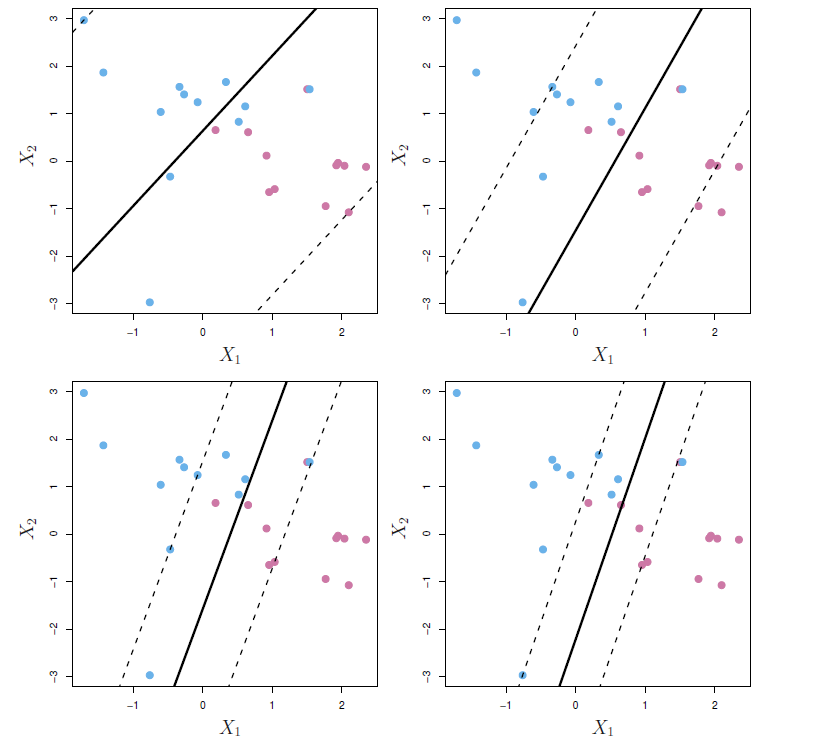
\includegraphics[scale=0.45]{images/regularization_parameter.png}
			\end{figure}
			
		\end{itemize}	
		
	}

	\section{Support Vector Machines}
	%%%%%%%%%%%%%%%%%%%%%%%%%%%%%%%%%%%%%%%%%%%%%%%%%%%%%%%%%%%%%%%%%%%
	\frame{\frametitle{The Need for Non-Linear Boundary}
		
		\begin{itemize}
			
			\item Linear boundary can fail in many cases, regardless of the value of C.
			\newline
			\begin{figure}
				\centering
				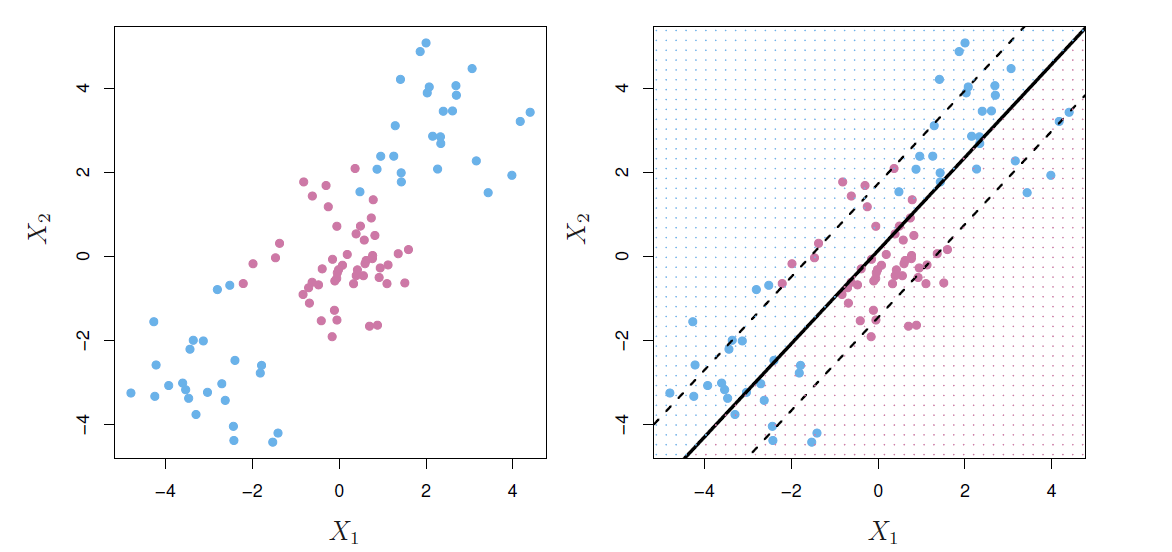
\includegraphics[scale=0.45]{images/non_linear_separable.png}
			\end{figure}
			
		\end{itemize}	
		
	}

		
	%%%%%%%%%%%%%%%%%%%%%%%%%%%%%%%%%%%%%%%%%%%%%%%%%%%%%%%%%%%%%%%%%%%
	\section{Conclusion}
	%%%%%%%%%%%%%%%%%%%%%%%%%%%%%%%%%%%%%%%%%%%%%%%%%%%%%%%%%%%%%%%%%%%
	\frame{\frametitle{Final Notes}
			\centering
			\vspace{50 pt}
			\textbf{Thank You!}
			\vspace{50pt}
			
			\textbf{Any Question?}
		}
	%%%%%%%%%%%%%%%%%%%%%%%%%%%%%%%%%%%%%%%%%%
\end{document}